\section{Aimspice plots} 


\begin{figure}[H]
    \centering
    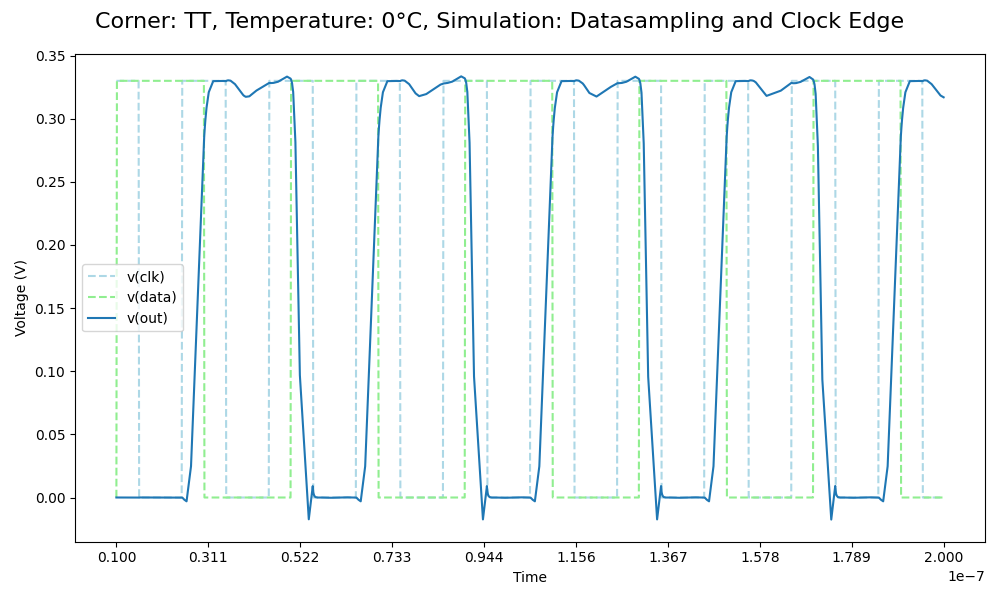
\includegraphics[height= 0.21\textheight]{figures/aimspice/TT/0/W1.csv.png}
    \vspace{5pt}
    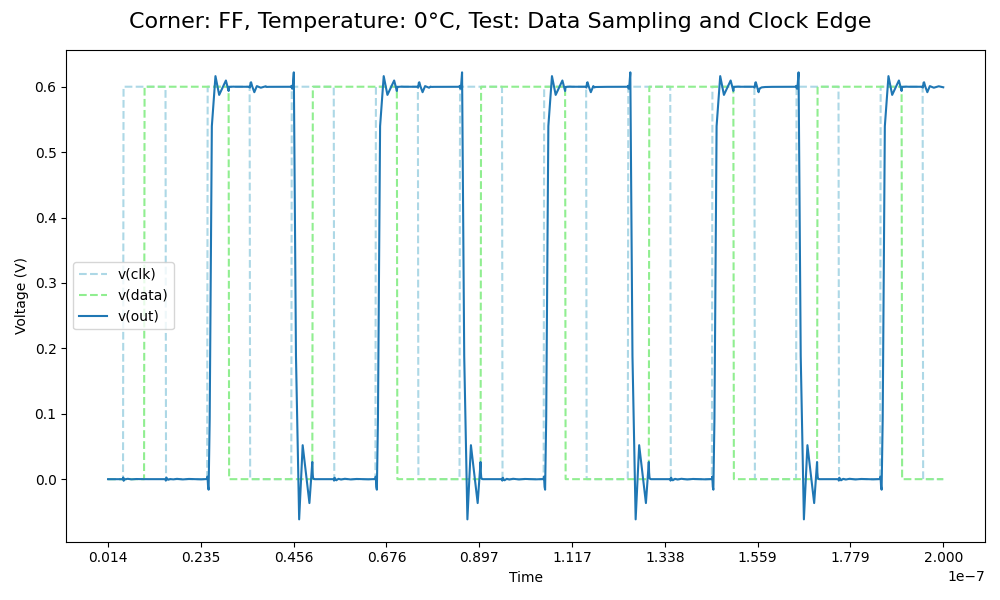
\includegraphics[height= 0.21\textheight]{figures/aimspice/FF/0/W1.csv.png}
    \vspace{5pt}
    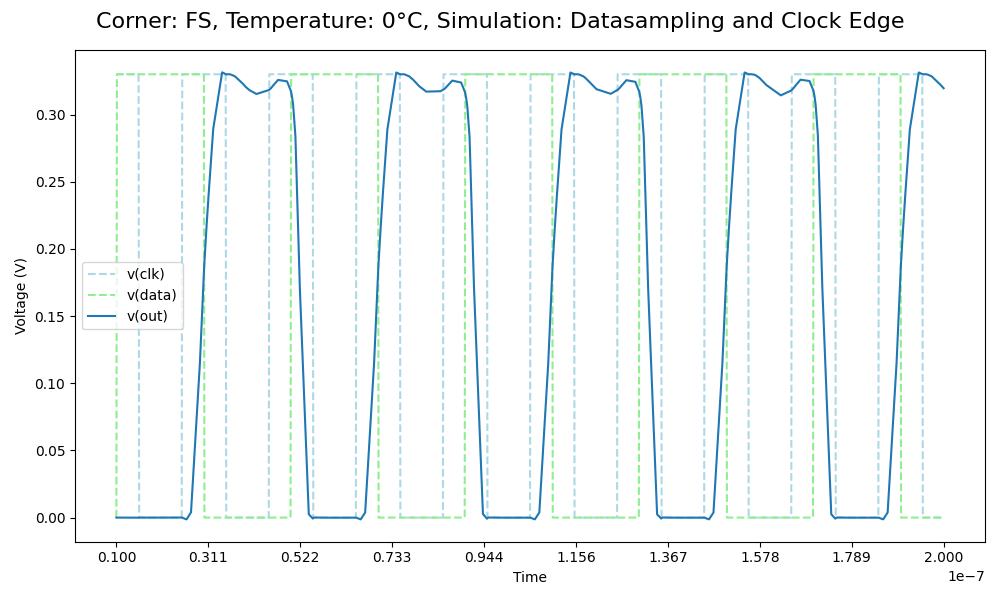
\includegraphics[height= 0.21\textheight]{figures/aimspice/FS/0/W1.csv.png}
    \vspace{5pt}
    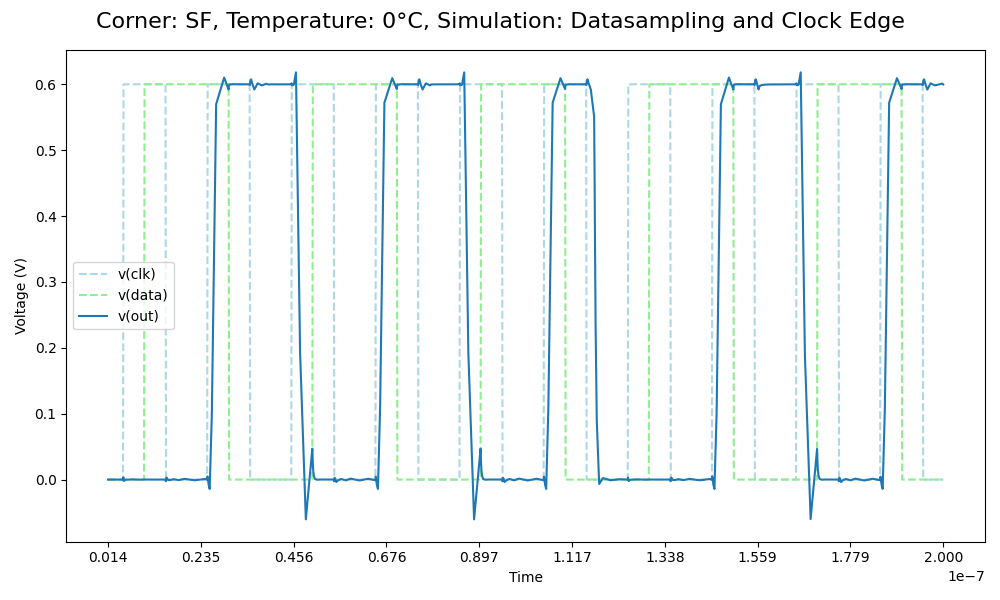
\includegraphics[height= 0.21\textheight]{figures/aimspice/SF/0/W1.csv.png}
    \vspace{5pt}
    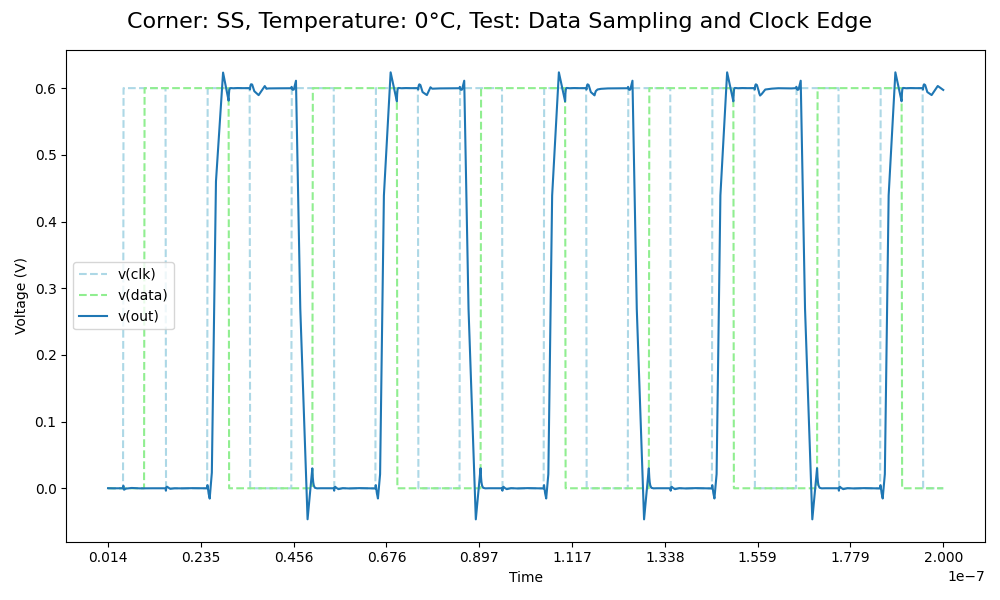
\includegraphics[height= 0.21\textheight]{figures/aimspice/SS/0/W1.csv.png}
    \caption{Test of datasampling at clock edge for 0 degrees Celsius.}
    \label{fig:aimspice_W1_0}
\end{figure}

\pagebreak

\begin{figure}[H]
    \centering
    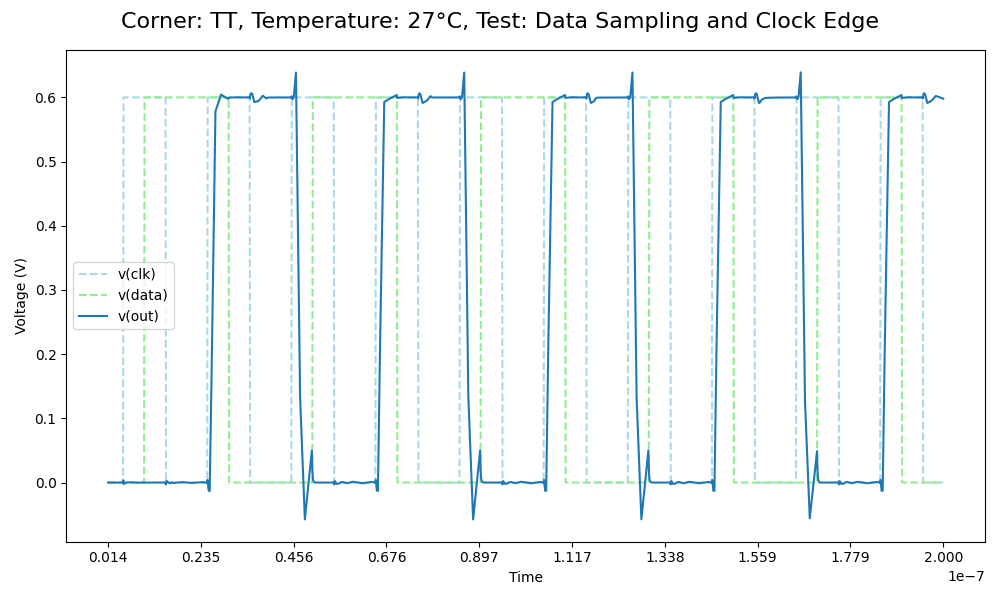
\includegraphics[height= 0.21\textheight]{figures/aimspice/TT/27/W1.csv.png}
    \vspace{5pt}
    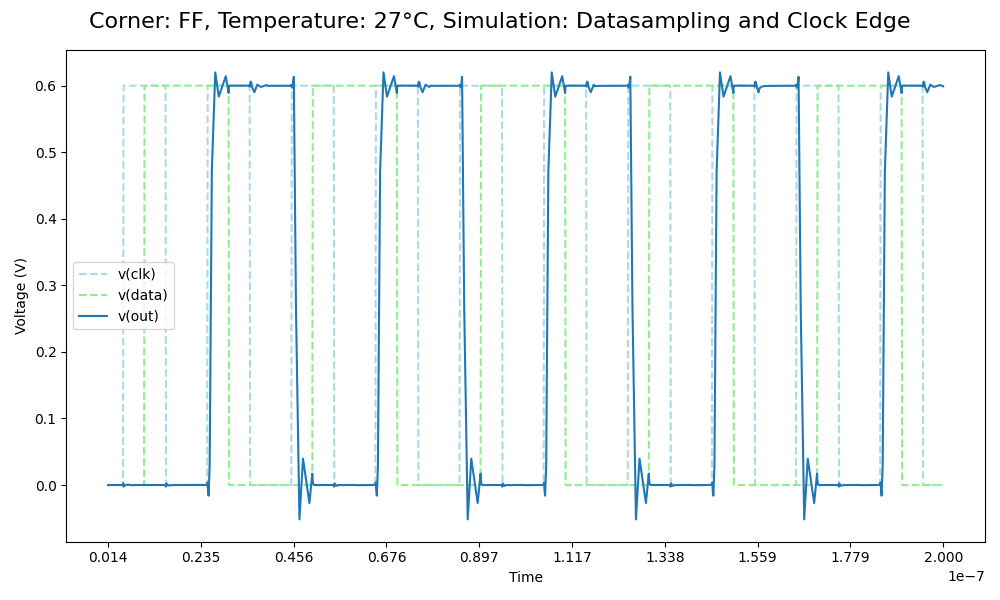
\includegraphics[height= 0.21\textheight]{figures/aimspice/FF/27/W1.csv.png}
    \vspace{5pt}
    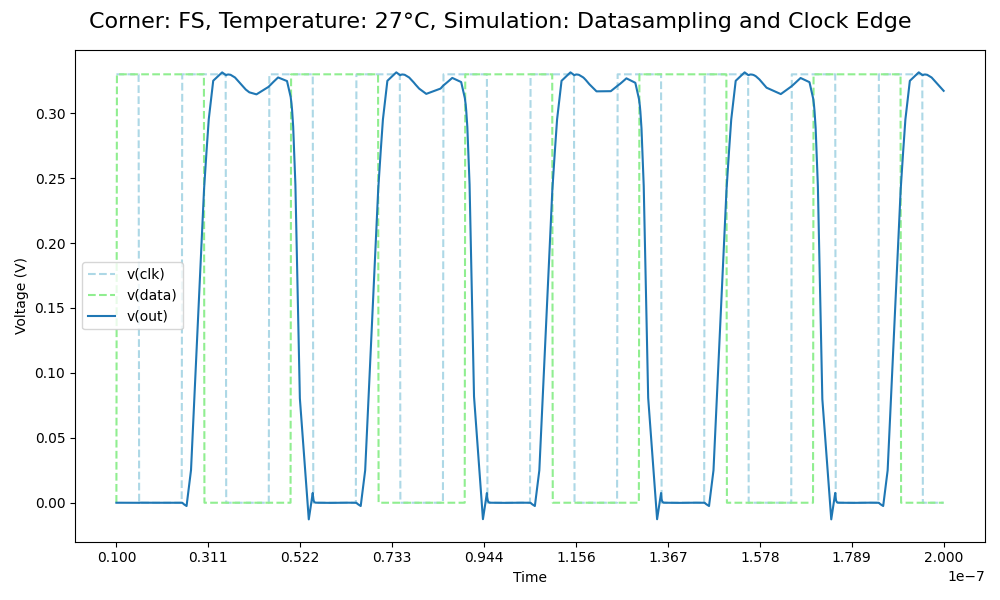
\includegraphics[height= 0.21\textheight]{figures/aimspice/FS/27/W1.csv.png}
    \vspace{5pt}
    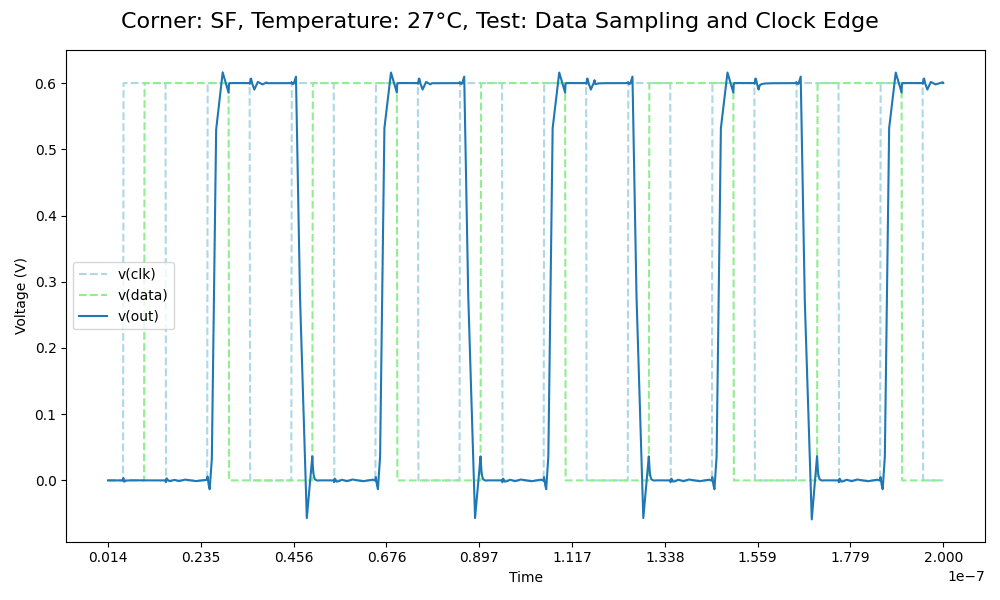
\includegraphics[height= 0.21\textheight]{figures/aimspice/SF/27/W1.csv.png}
    \vspace{5pt}
    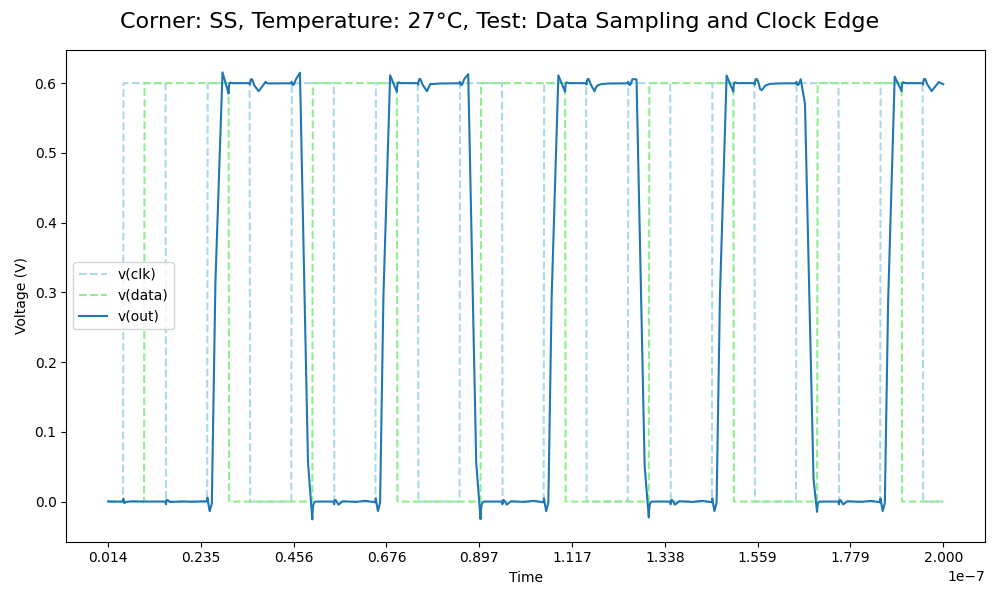
\includegraphics[height= 0.21\textheight]{figures/aimspice/SS/27/W1.csv.png}
    \caption{Test of datasampling at clock edge for 27 degrees Celsius.}
    \label{fig:aimspice_W1_27}
\end{figure}

\pagebreak

\begin{figure}[H]
    \centering
    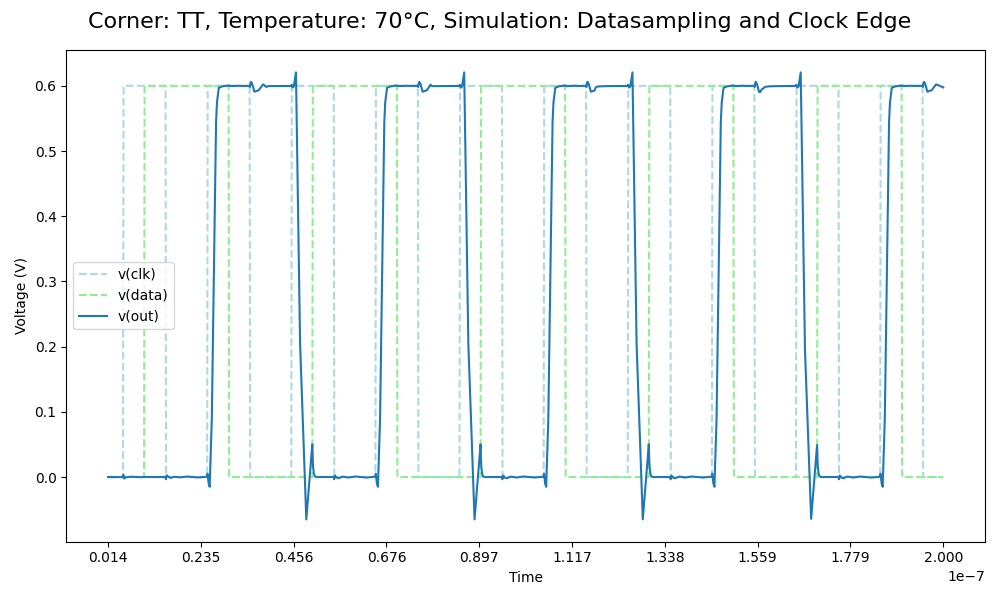
\includegraphics[height= 0.21\textheight]{figures/aimspice/TT/70/W1.csv.png}
    \vspace{5pt}
    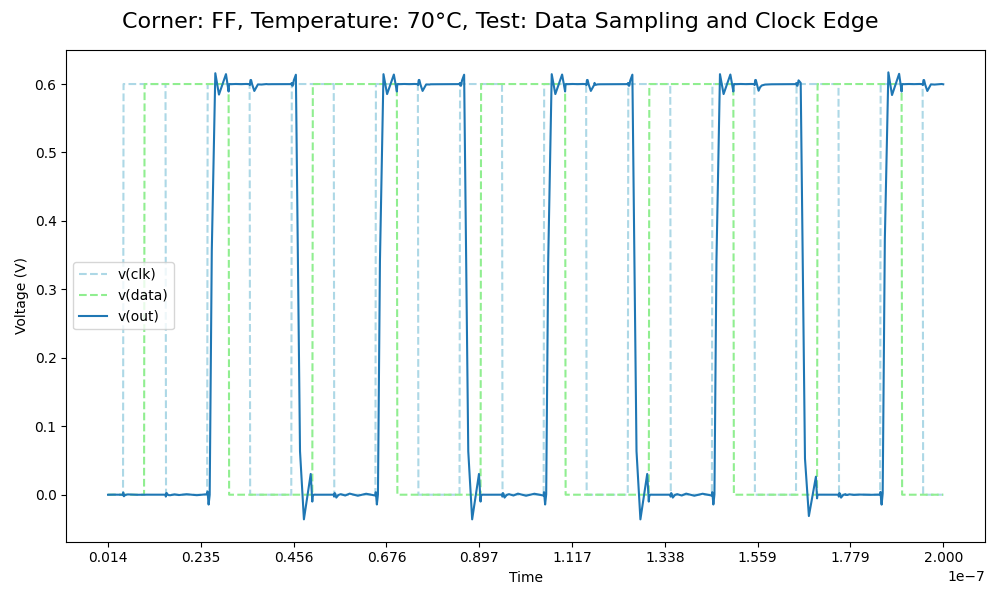
\includegraphics[height= 0.21\textheight]{figures/aimspice/FF/70/W1.csv.png}
    \vspace{5pt}
    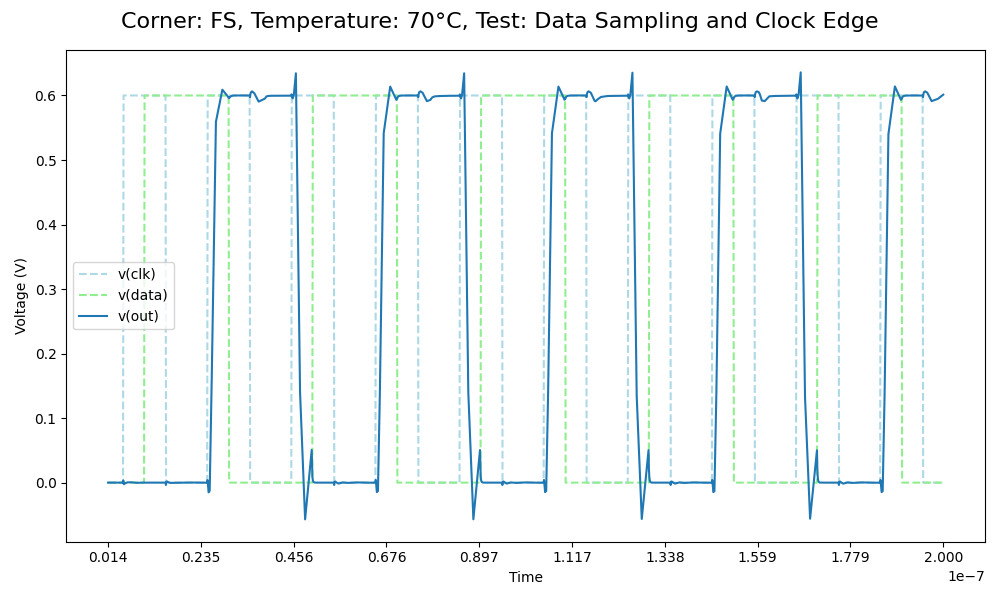
\includegraphics[height= 0.21\textheight]{figures/aimspice/FS/70/W1.csv.png}
    \vspace{5pt}
    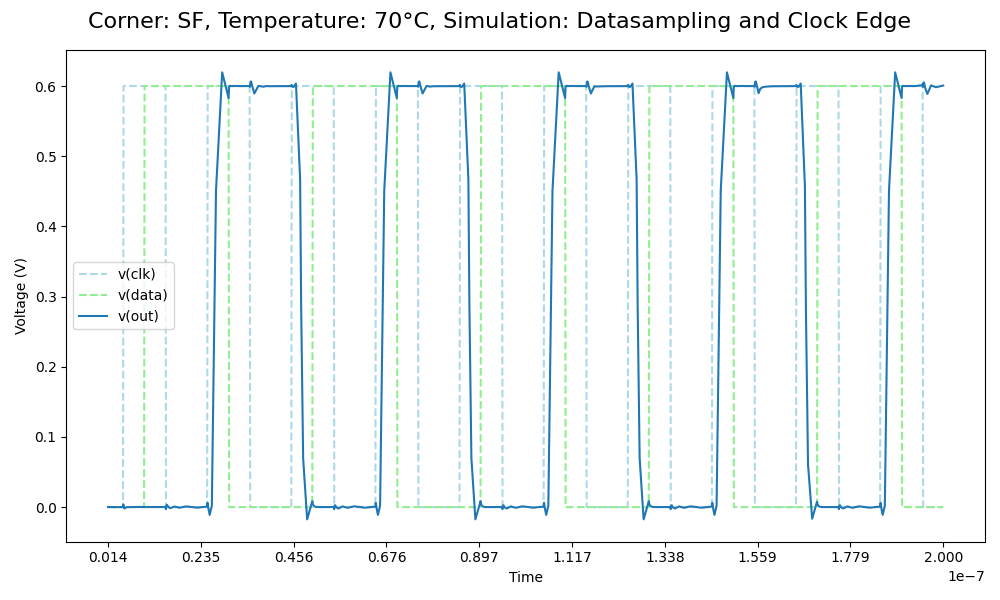
\includegraphics[height= 0.21\textheight]{figures/aimspice/SF/70/W1.csv.png}
    \vspace{5pt}
    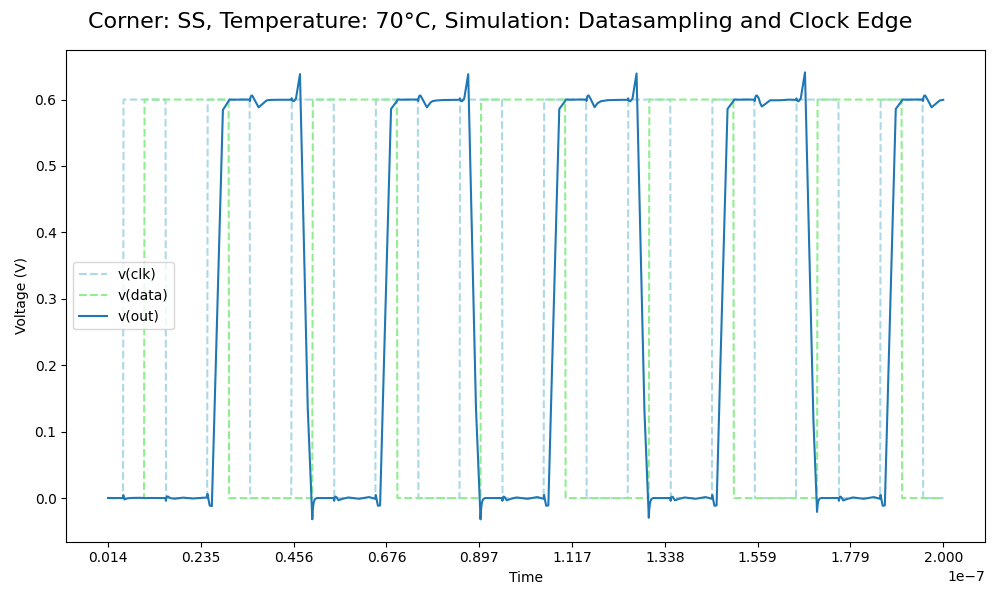
\includegraphics[height= 0.21\textheight]{figures/aimspice/SS/70/W1.csv.png}
    \caption{Test of datasampling at clock edge for 70 degrees Celsius.}
    \label{fig:aimspice_W1_70}
\end{figure}

\pagebreak

\begin{figure}[H]
    \centering
    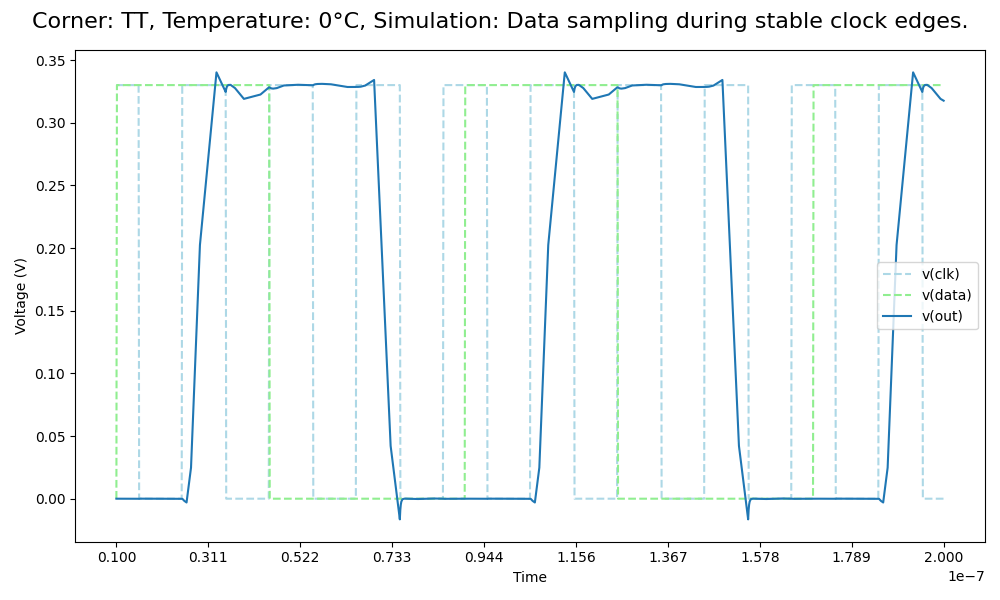
\includegraphics[height= 0.21\textheight]{figures/aimspice/TT/0/W2.csv.png}
    \vspace{5pt}
    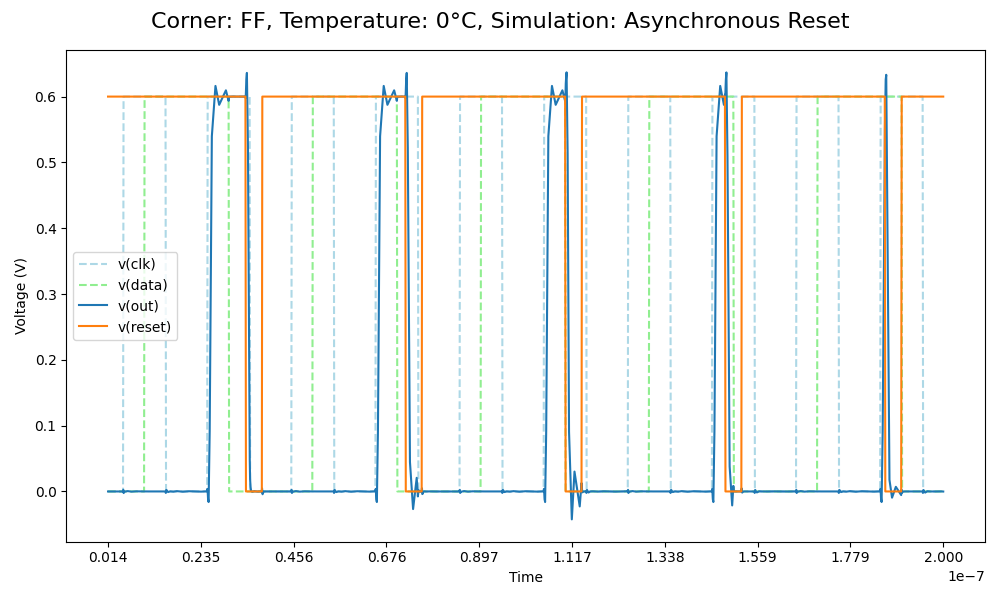
\includegraphics[height= 0.21\textheight]{figures/aimspice/FF/0/W2.csv.png}
    \vspace{5pt}
    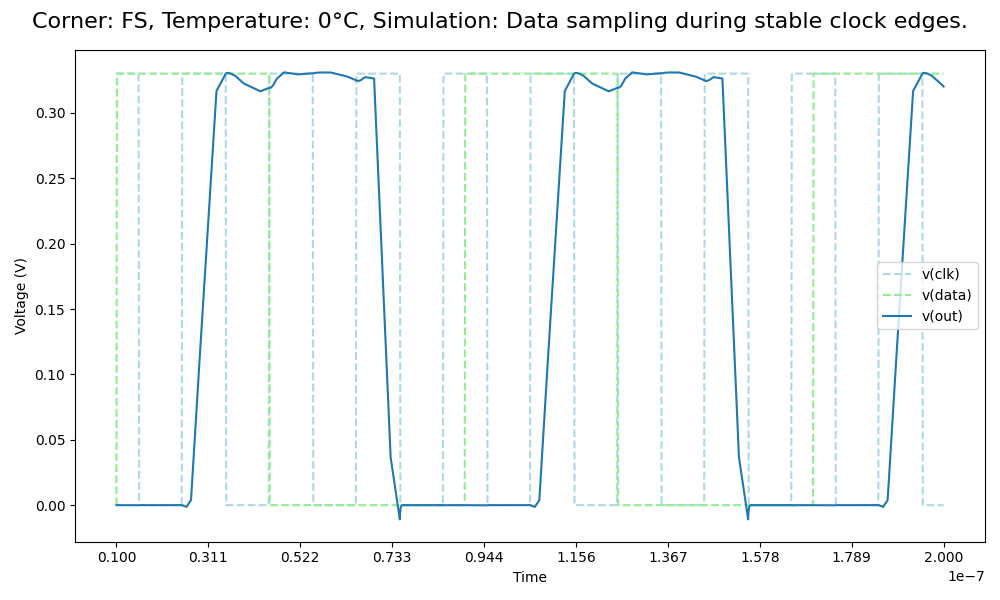
\includegraphics[height= 0.21\textheight]{figures/aimspice/FS/0/W2.csv.png}
    \vspace{5pt}
    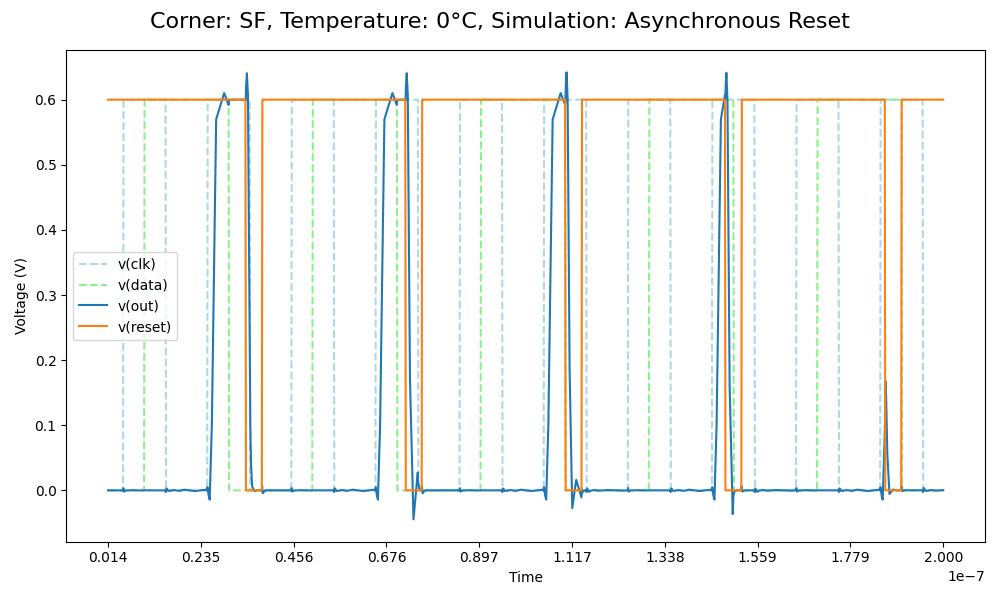
\includegraphics[height= 0.21\textheight]{figures/aimspice/SF/0/W2.csv.png}
    \vspace{5pt}
    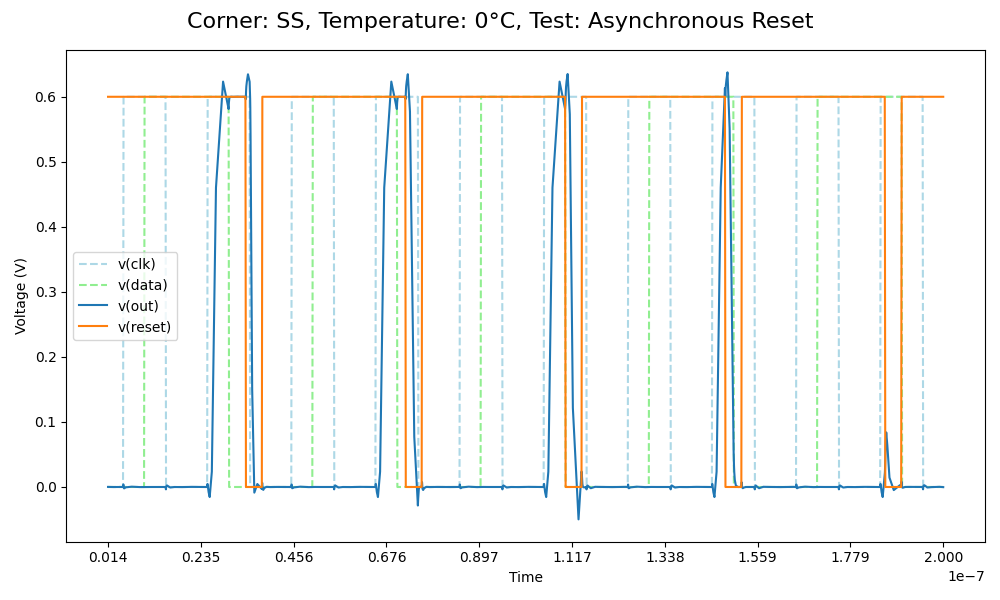
\includegraphics[height= 0.21\textheight]{figures/aimspice/SS/0/W2.csv.png}
    \caption{Test of the asyncrhronous reset for 0 degrees celcius.}
    \label{fig:aimspice_W2_0}
\end{figure}

\pagebreak

\begin{figure}[H]
    \centering
    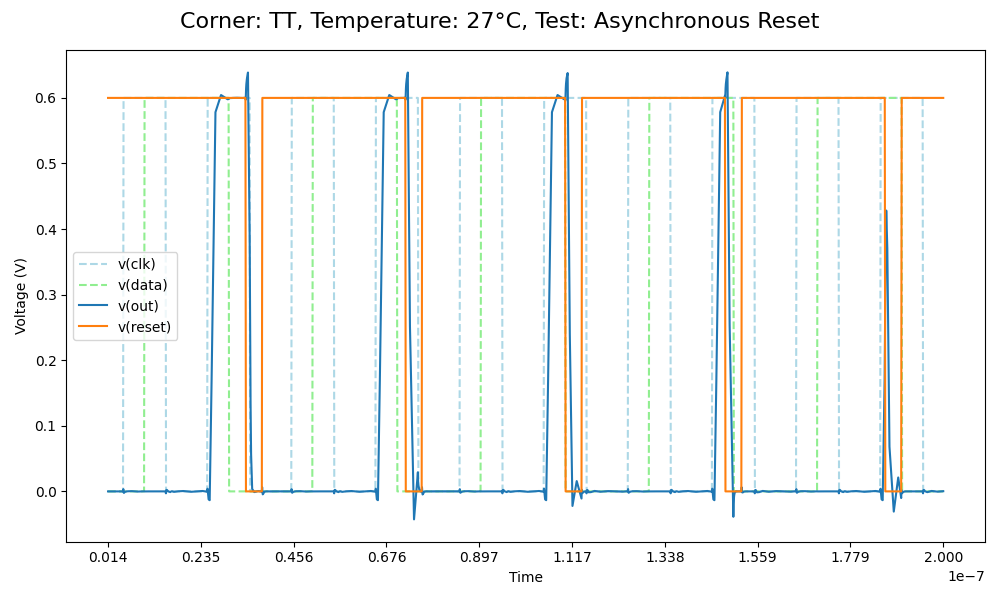
\includegraphics[height= 0.21\textheight]{figures/aimspice/TT/27/W2.csv.png}
    \vspace{5pt}
    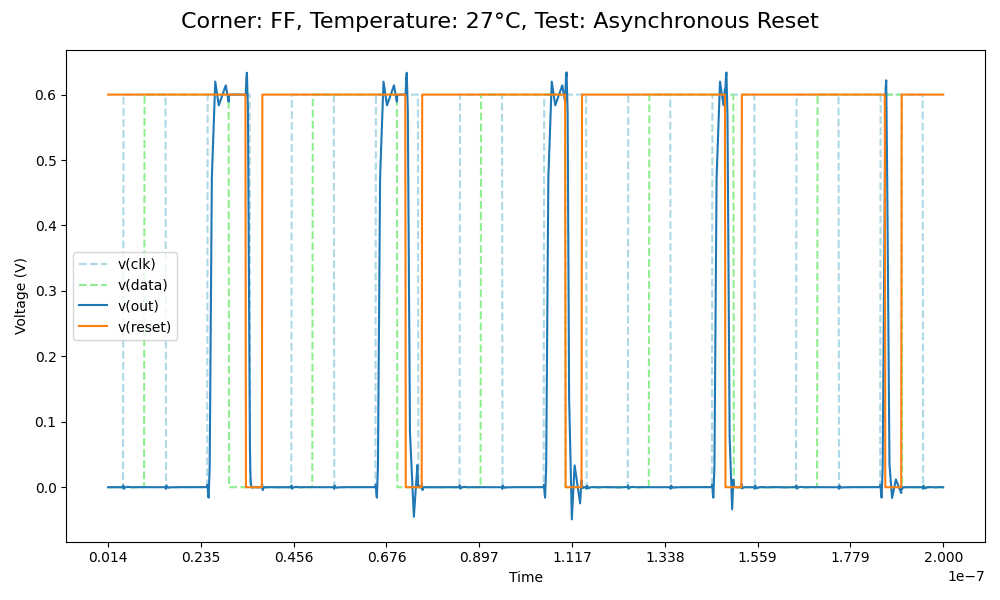
\includegraphics[height= 0.21\textheight]{figures/aimspice/FF/27/W2.csv.png}
    \vspace{5pt}
    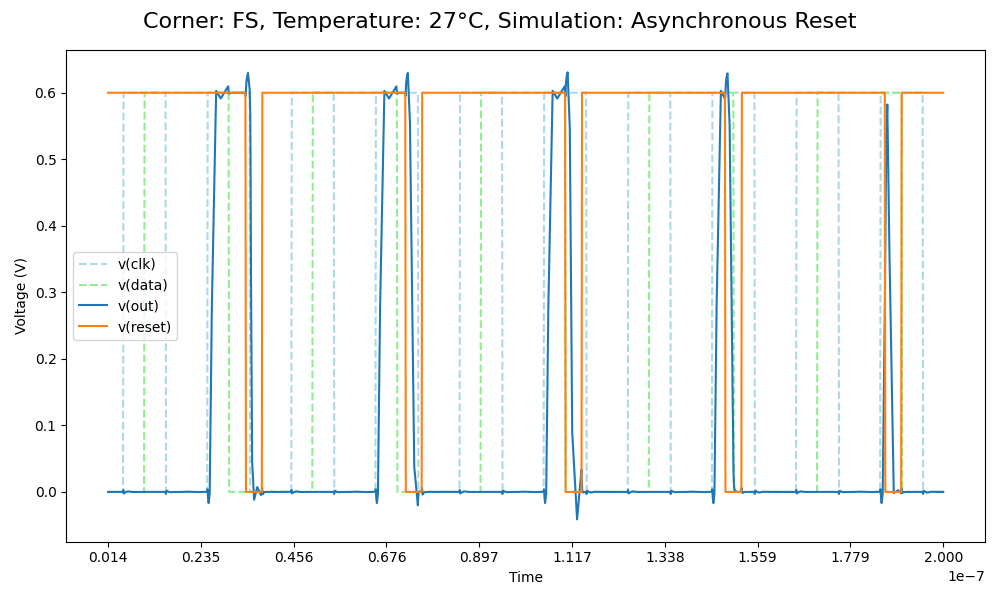
\includegraphics[height= 0.21\textheight]{figures/aimspice/FS/27/W2.csv.png}
    \vspace{5pt}
    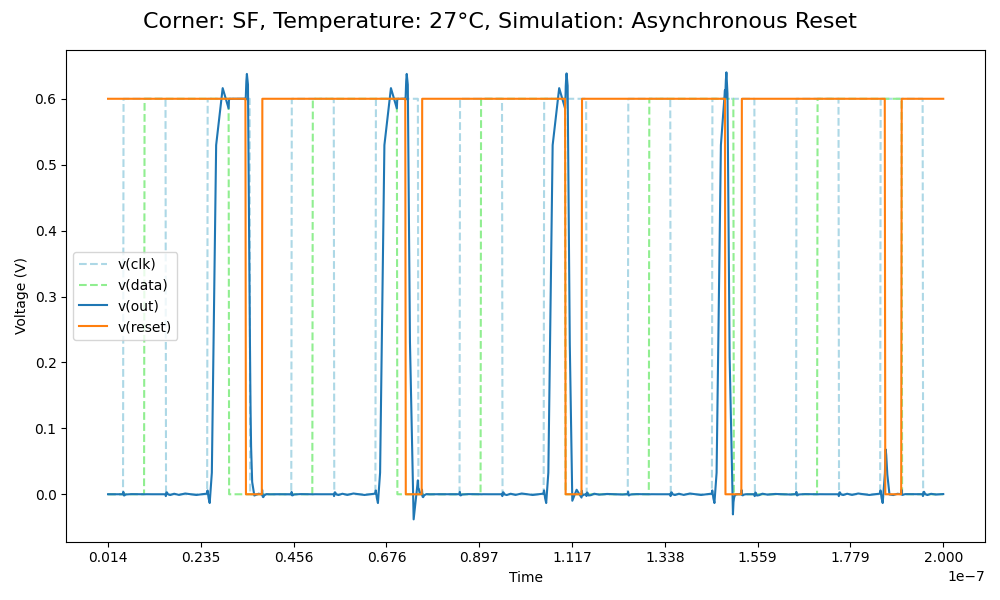
\includegraphics[height= 0.21\textheight]{figures/aimspice/SF/27/W2.csv.png}
    \vspace{5pt}
    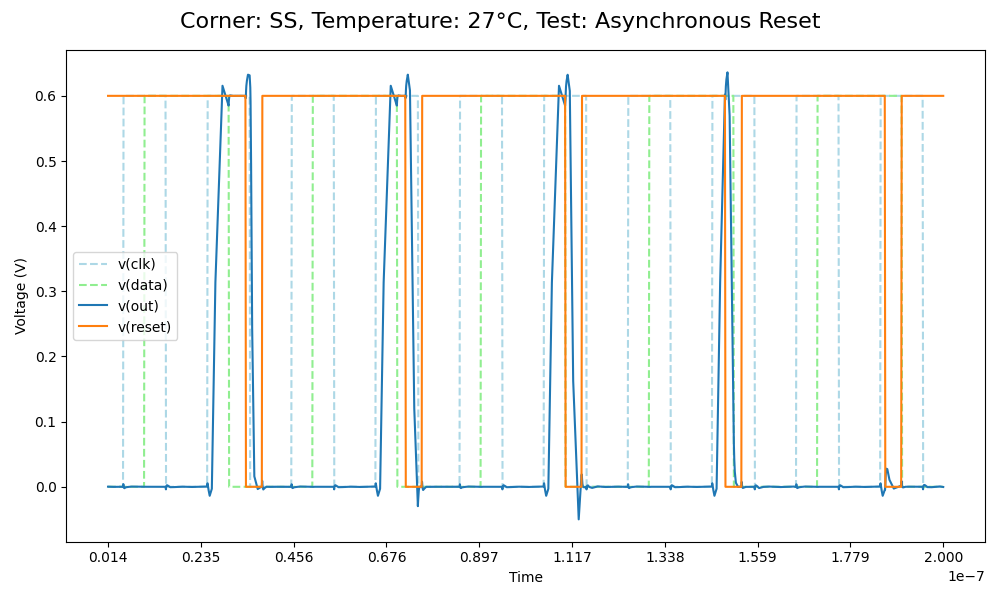
\includegraphics[height= 0.21\textheight]{figures/aimspice/SS/27/W2.csv.png}
    \caption{Test of the asyncrhronous reset for 27 degrees celcius.}
    \label{fig:aimspice_W2_27}
\end{figure}

\pagebreak

\begin{figure}[H]
    \centering
    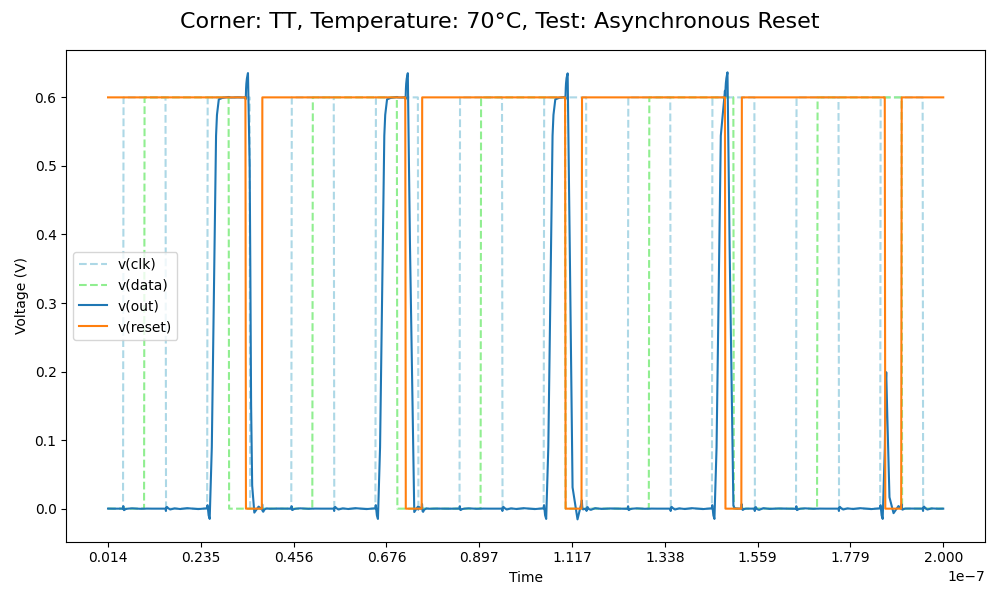
\includegraphics[height= 0.21\textheight]{figures/aimspice/TT/70/W2.csv.png}
    \vspace{5pt}
    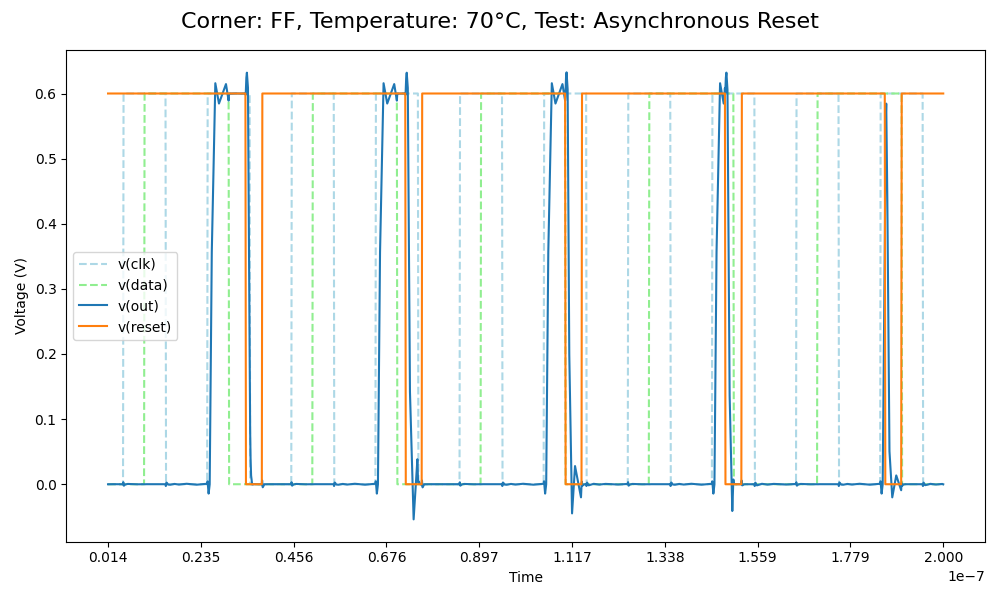
\includegraphics[height= 0.21\textheight]{figures/aimspice/FF/70/W2.csv.png}
    \vspace{5pt}
    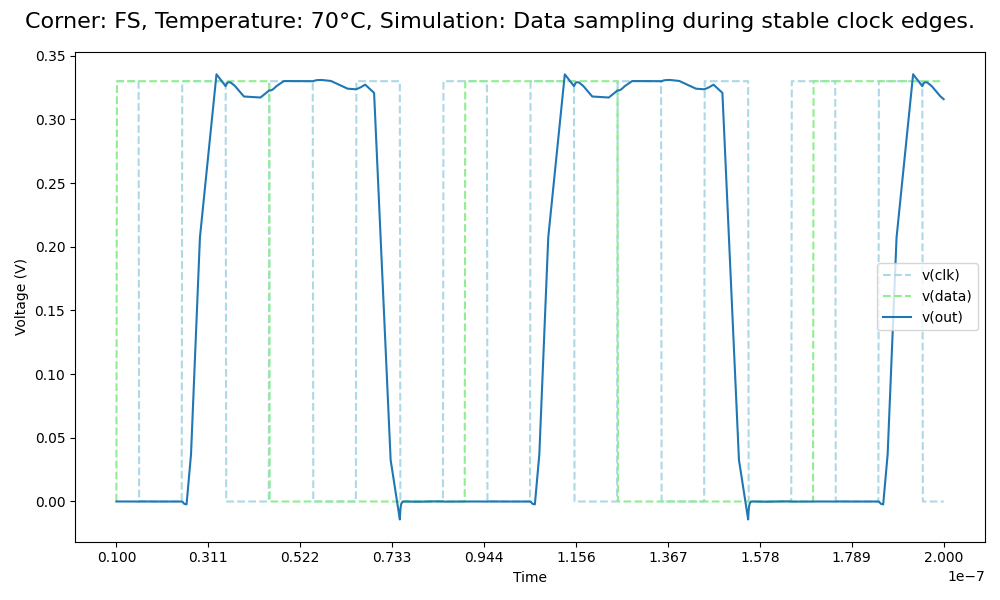
\includegraphics[height= 0.21\textheight]{figures/aimspice/FS/70/W2.csv.png}
    \vspace{5pt}
    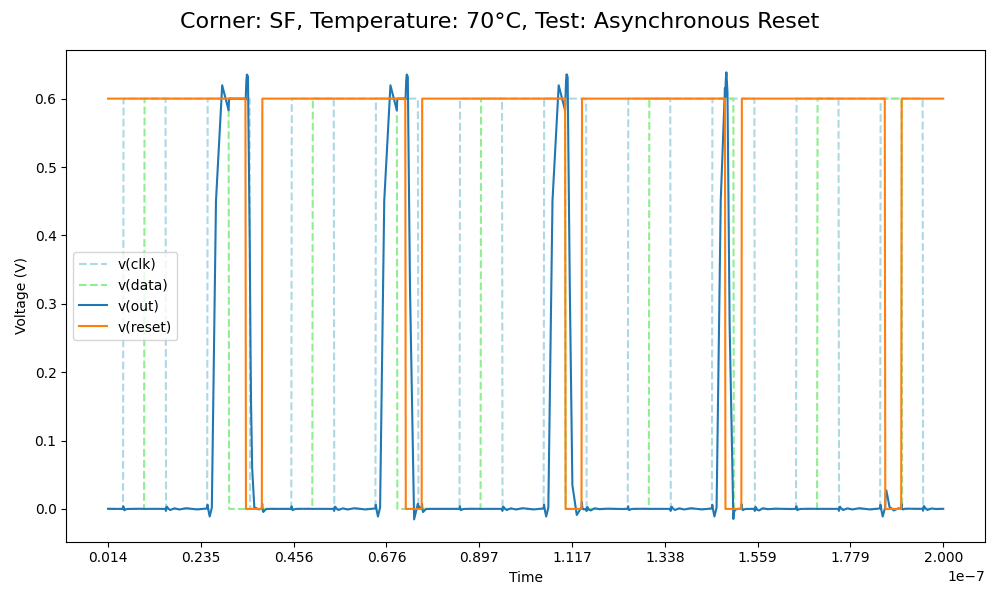
\includegraphics[height= 0.21\textheight]{figures/aimspice/SF/70/W2.csv.png}
    \vspace{5pt}
    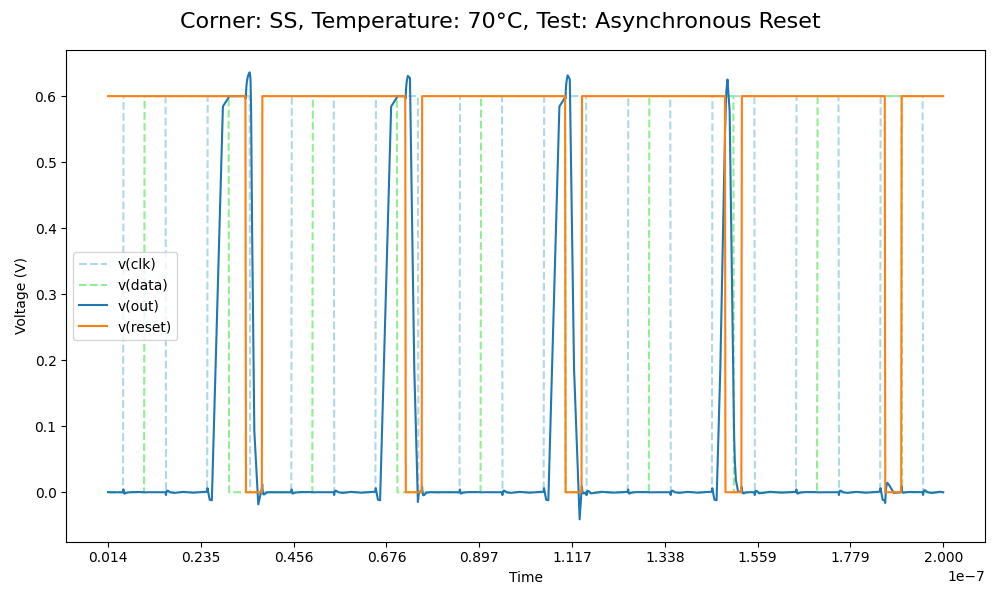
\includegraphics[height= 0.21\textheight]{figures/aimspice/SS/70/W2.csv.png}
    \caption{Test of the asyncrhronous reset for 70 degrees celcius.}
    \label{fig:aimspice_W2_70}
\end{figure}

\pagebreak

\begin{figure}[H]
    \centering
    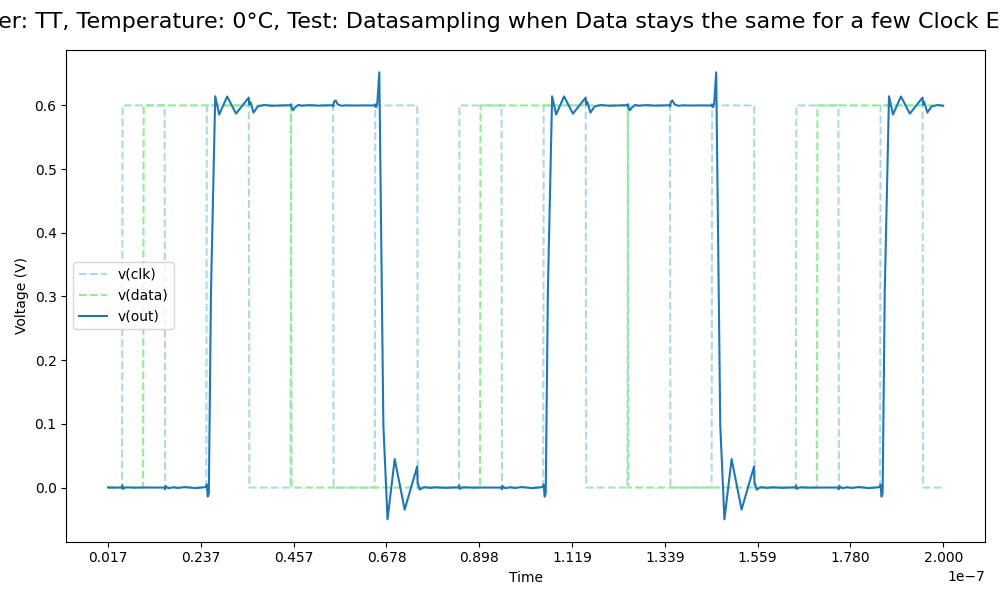
\includegraphics[height= 0.21\textheight]{figures/aimspice/TT/0/W3.csv.png}
    \vspace{5pt}
    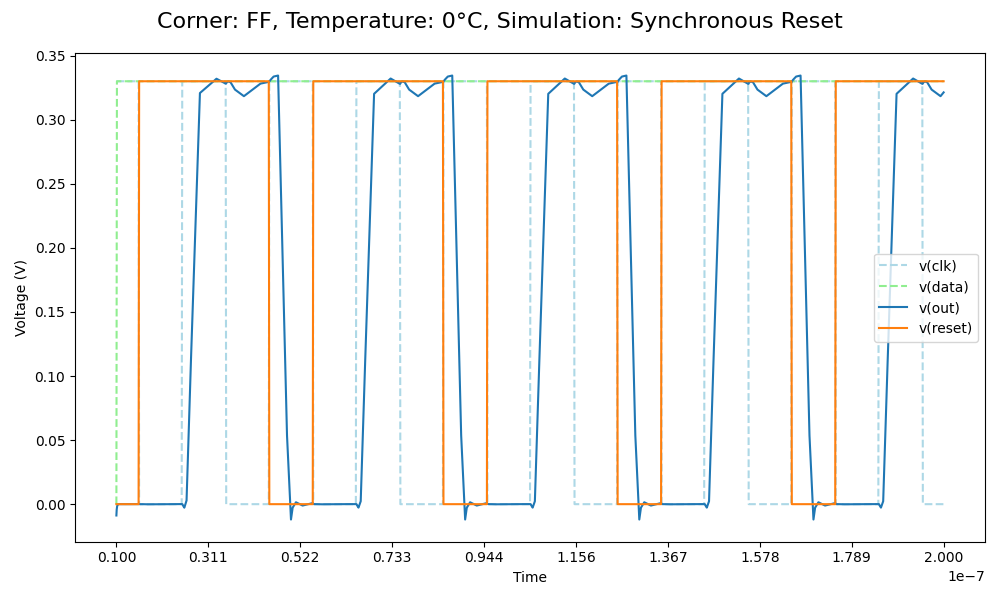
\includegraphics[height= 0.21\textheight]{figures/aimspice/FF/0/W3.csv.png}
    \vspace{5pt}
    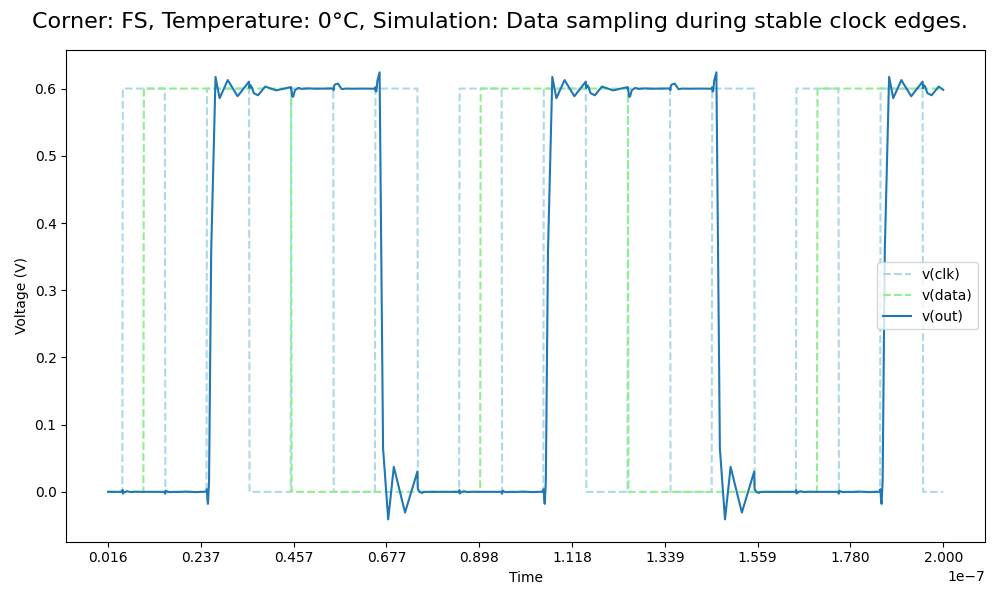
\includegraphics[height= 0.21\textheight]{figures/aimspice/FS/0/W3.csv.png}
    \vspace{5pt}
    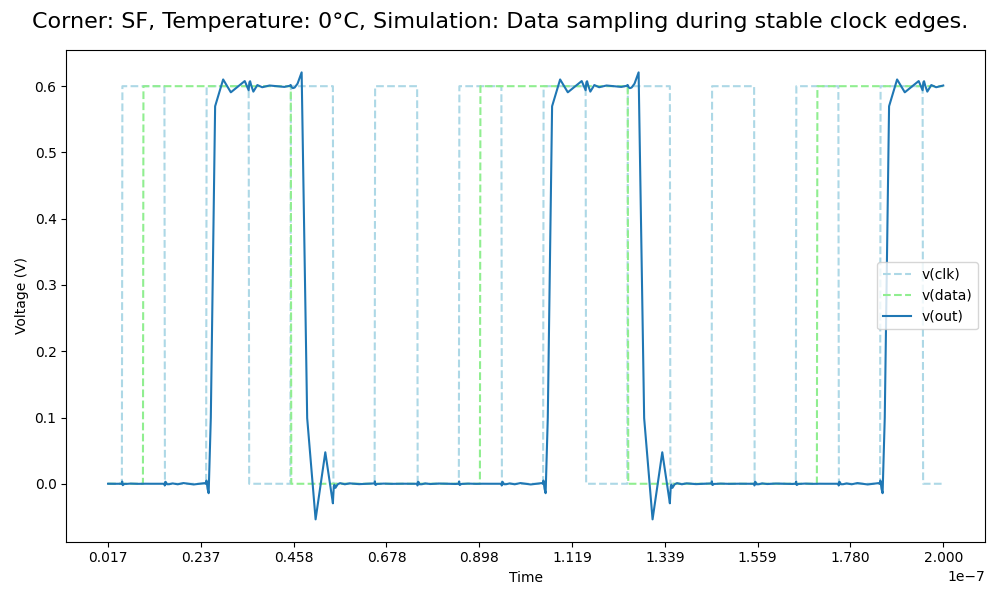
\includegraphics[height= 0.21\textheight]{figures/aimspice/SF/0/W3.csv.png}
    \vspace{5pt}
    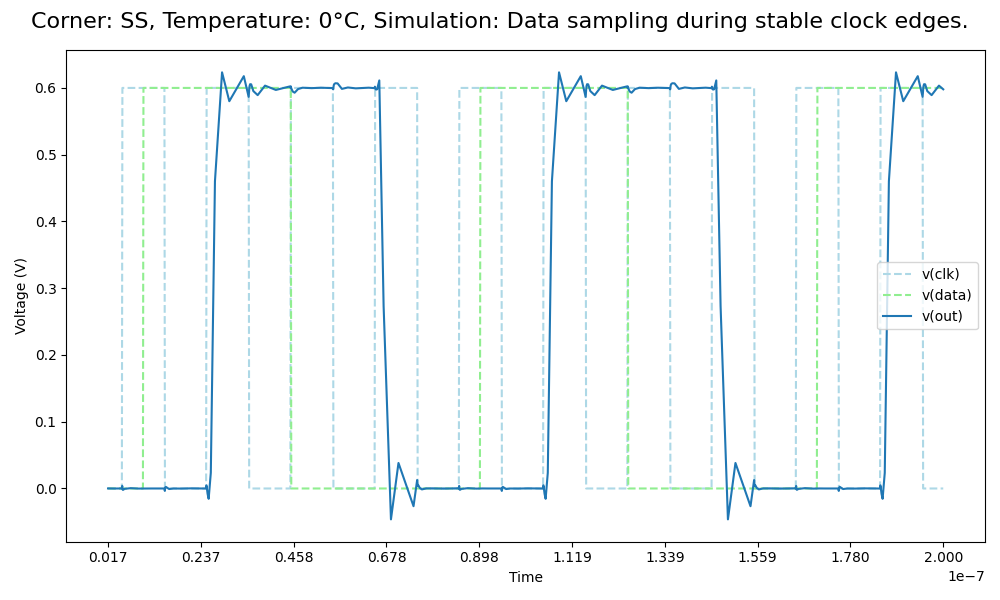
\includegraphics[height= 0.21\textheight]{figures/aimspice/SS/0/W3.csv.png}
    \caption{Test of datasampling when the data stays the same for a few clock edges at 0 degrees celcius.}
    \label{fig:aimspice_W3_0}
\end{figure}

\pagebreak

\begin{figure}[H]
    \centering
    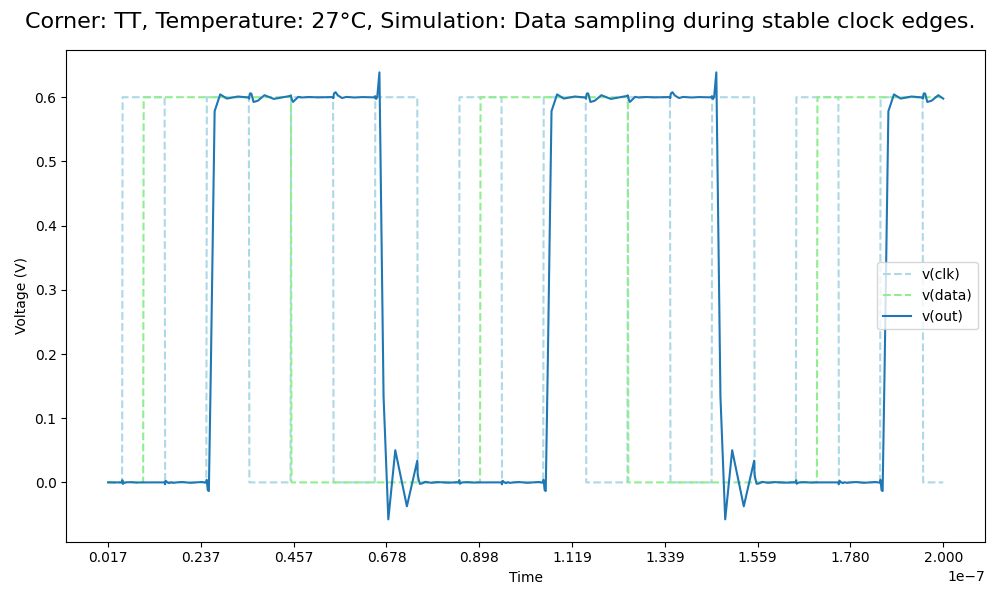
\includegraphics[height= 0.21\textheight]{figures/aimspice/TT/27/W3.csv.png}
    \vspace{5pt}
    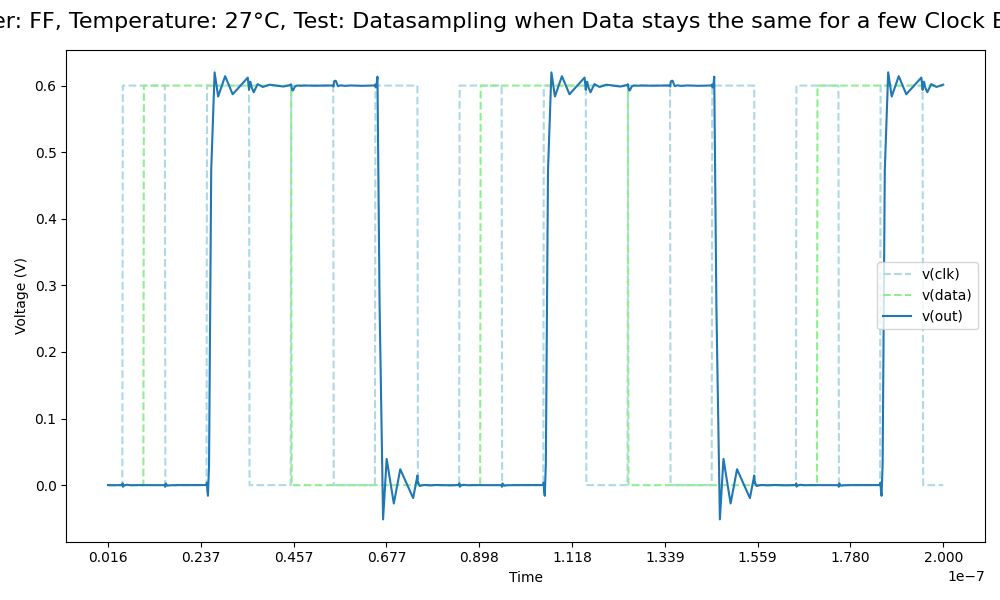
\includegraphics[height= 0.21\textheight]{figures/aimspice/FF/27/W3.csv.png}
    \vspace{5pt}
    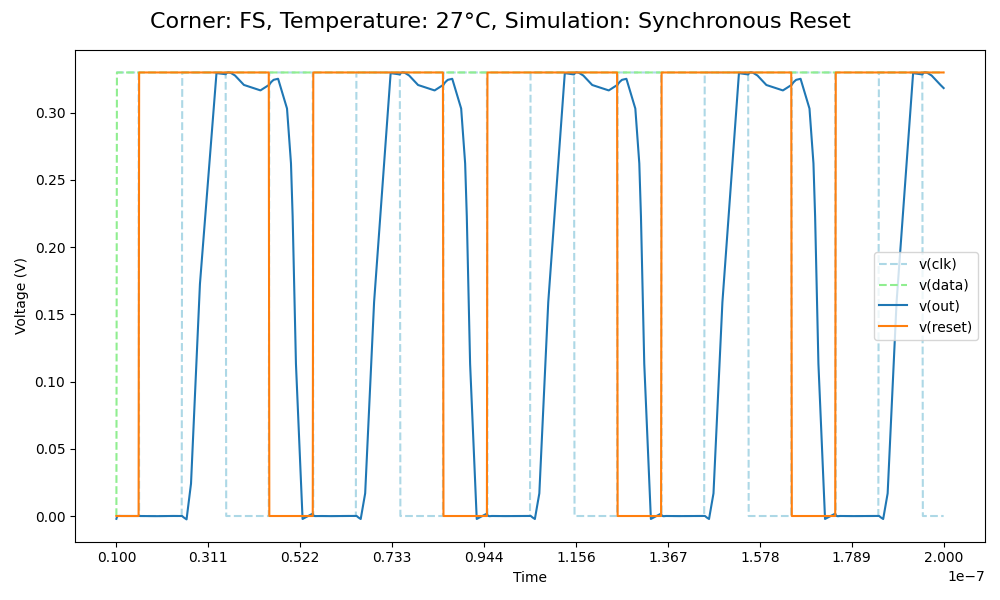
\includegraphics[height= 0.21\textheight]{figures/aimspice/FS/27/W3.csv.png}
    \vspace{5pt}
    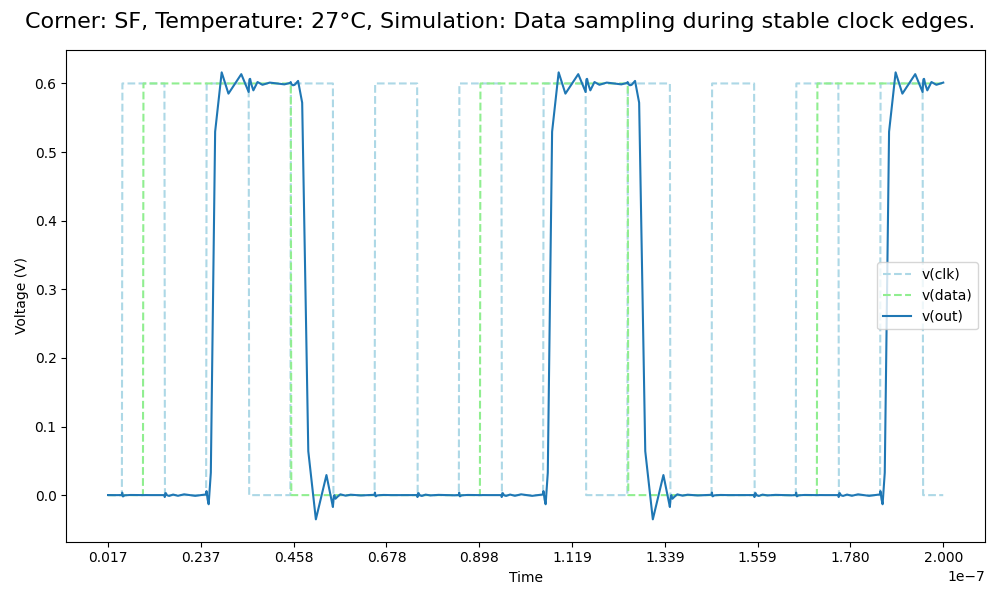
\includegraphics[height= 0.21\textheight]{figures/aimspice/SF/27/W3.csv.png}
    \vspace{5pt}
    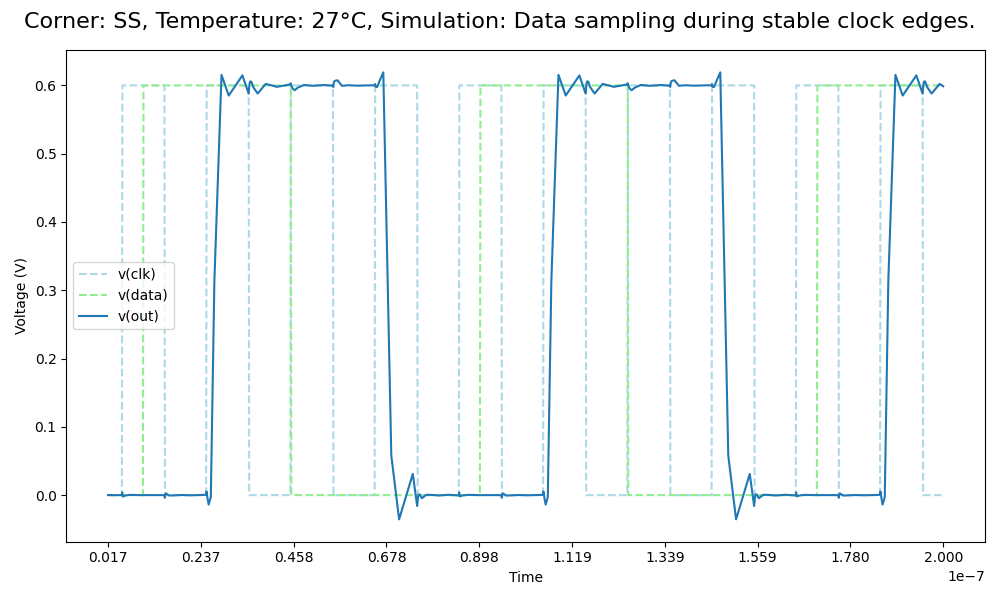
\includegraphics[height= 0.21\textheight]{figures/aimspice/SS/27/W3.csv.png}
    \caption{Test of datasampling when the data stays the same for a few clock edges at 27 degrees celcius.}
    \label{fig:aimspice_W3_27}
\end{figure}

\pagebreak

\begin{figure}[H]
    \centering
    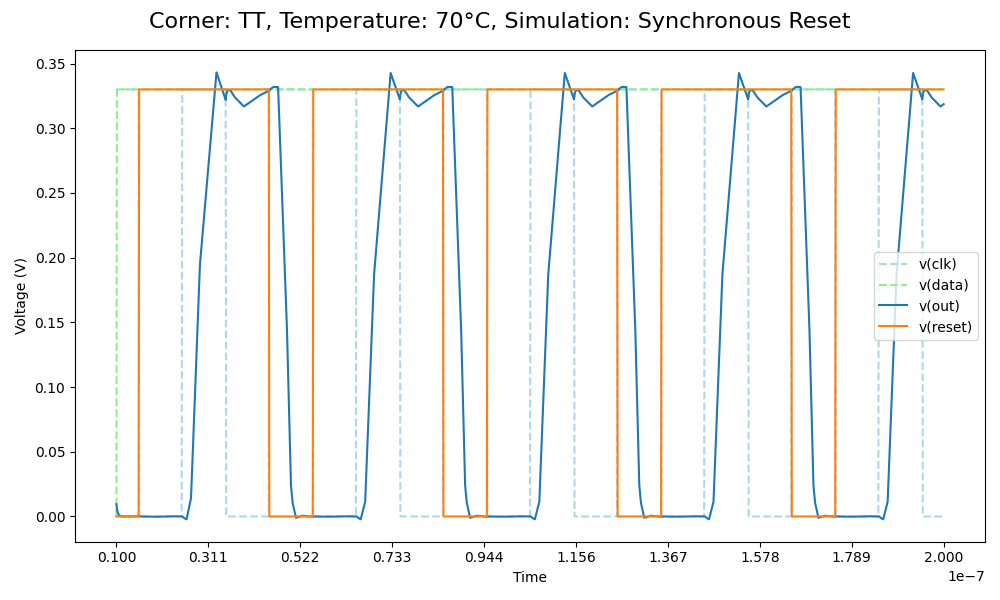
\includegraphics[height= 0.21\textheight]{figures/aimspice/TT/70/W3.csv.png}
    \vspace{5pt}
    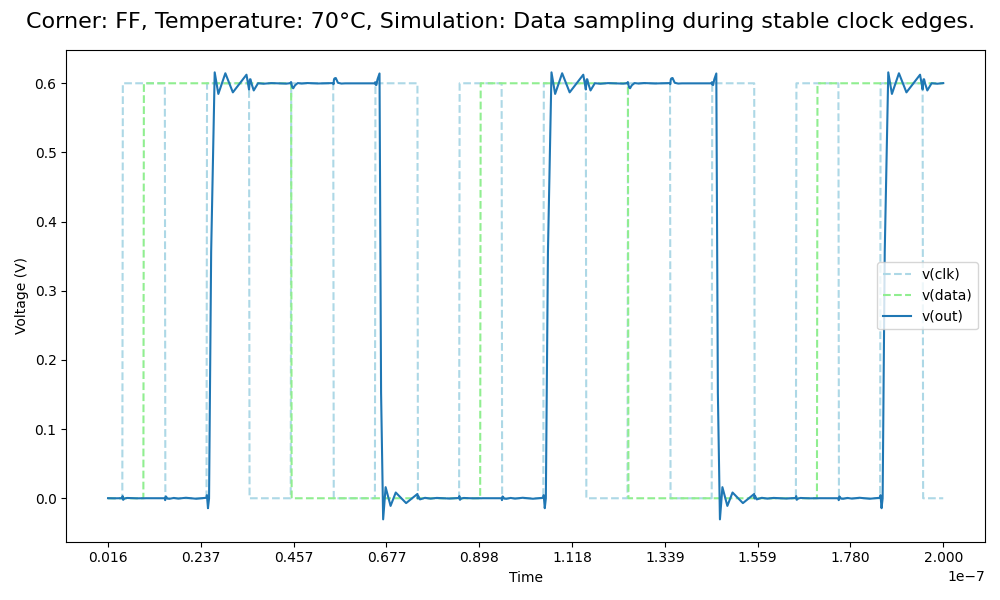
\includegraphics[height= 0.21\textheight]{figures/aimspice/FF/70/W3.csv.png}
    \vspace{5pt}
    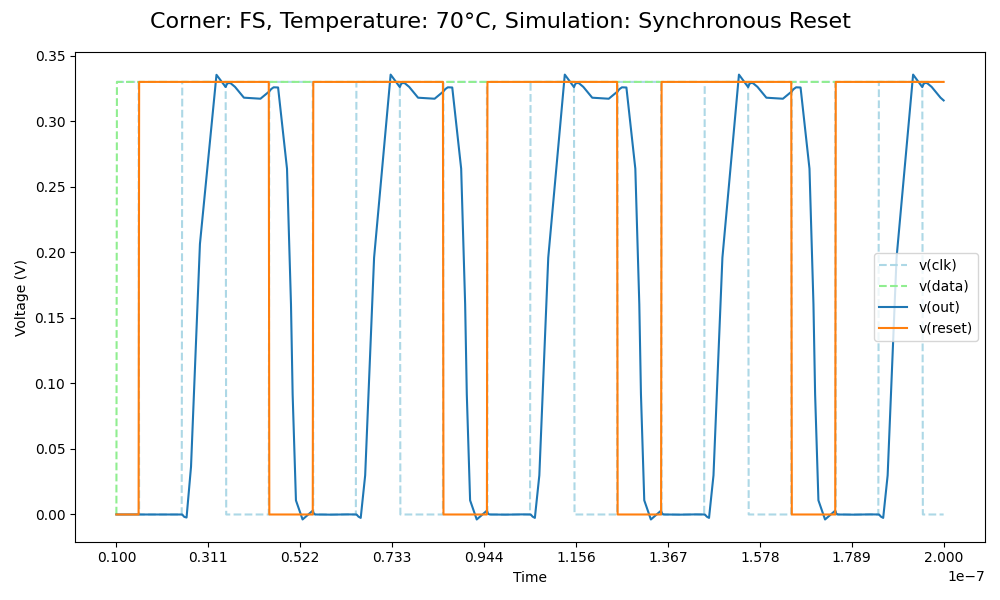
\includegraphics[height= 0.21\textheight]{figures/aimspice/FS/70/W3.csv.png}
    \vspace{5pt}
    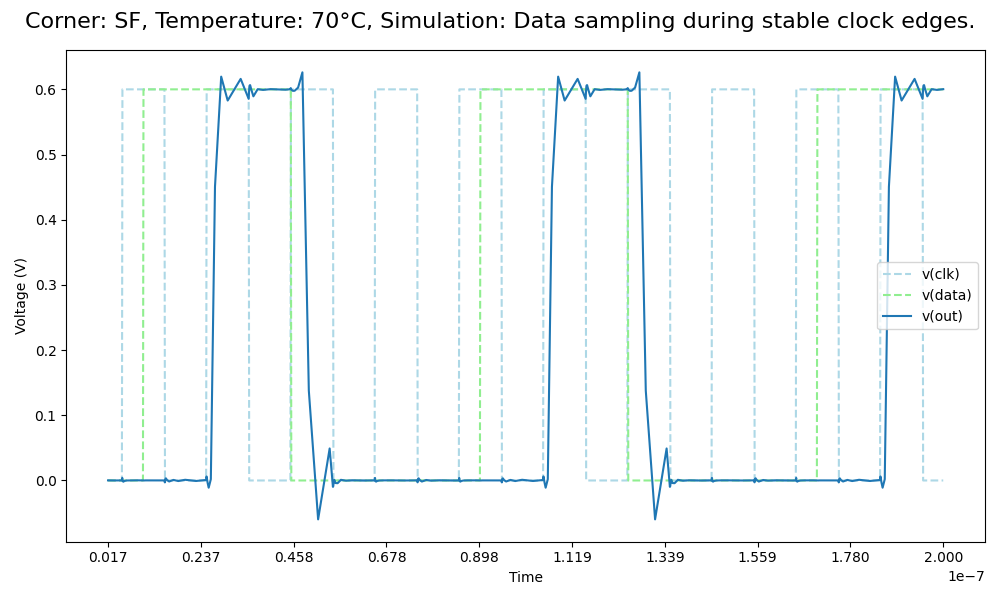
\includegraphics[height= 0.21\textheight]{figures/aimspice/SF/70/W3.csv.png}
    \vspace{5pt}
    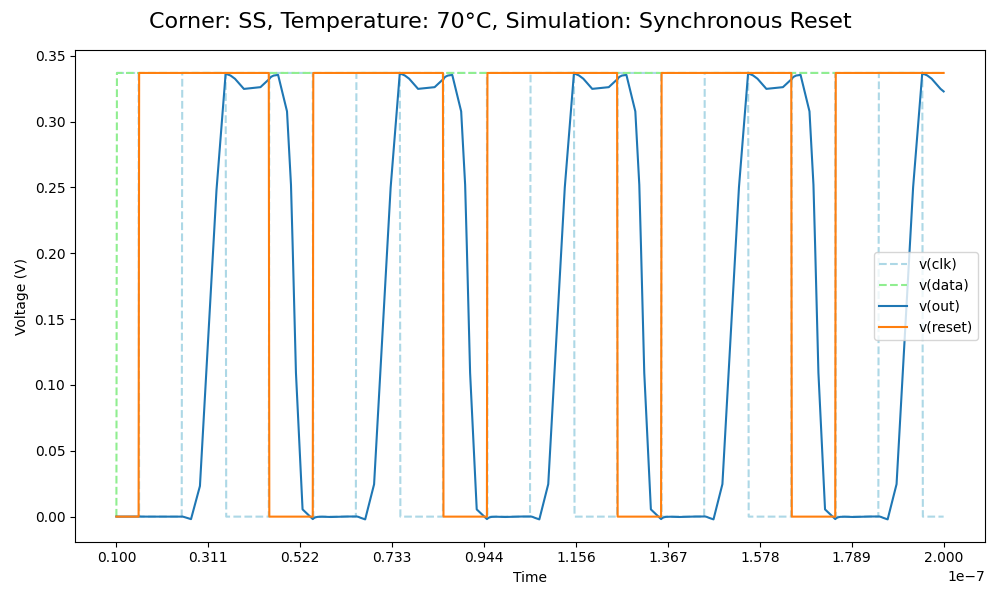
\includegraphics[height= 0.21\textheight]{figures/aimspice/SS/70/W3.csv.png}
    \caption{Test of datasampling when the data stays the same for a few clock edges at 70 degrees celcius.}
    \label{fig:aimspice_W3_70}
\end{figure}

\pagebreak


\begin{figure}[H]
    \centering
    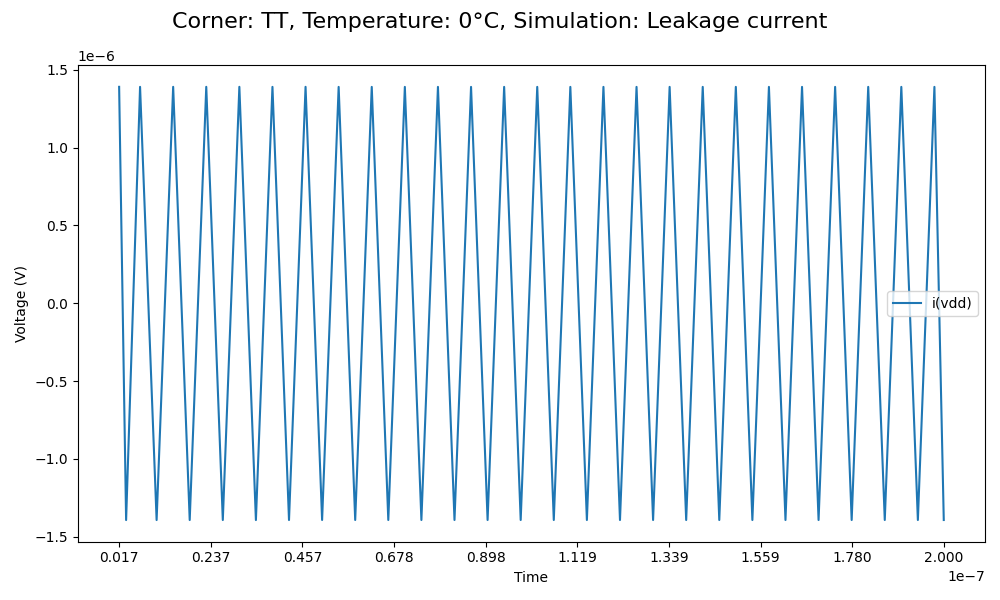
\includegraphics[height= 0.21\textheight]{figures/aimspice/TT/0/I.csv.png}
    \vspace{5pt}
    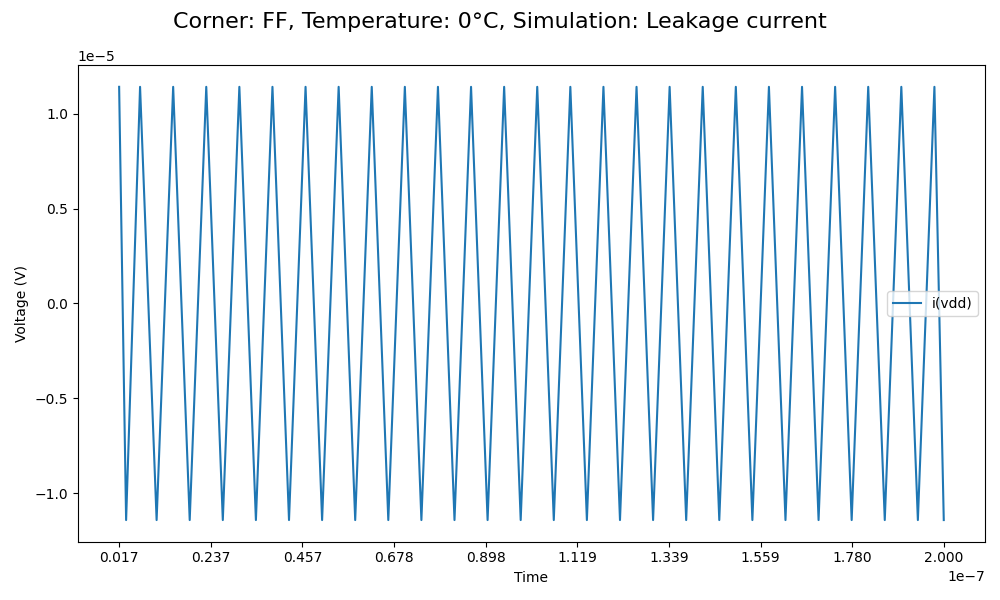
\includegraphics[height= 0.21\textheight]{figures/aimspice/FF/0/I.csv.png}
    \vspace{5pt}
    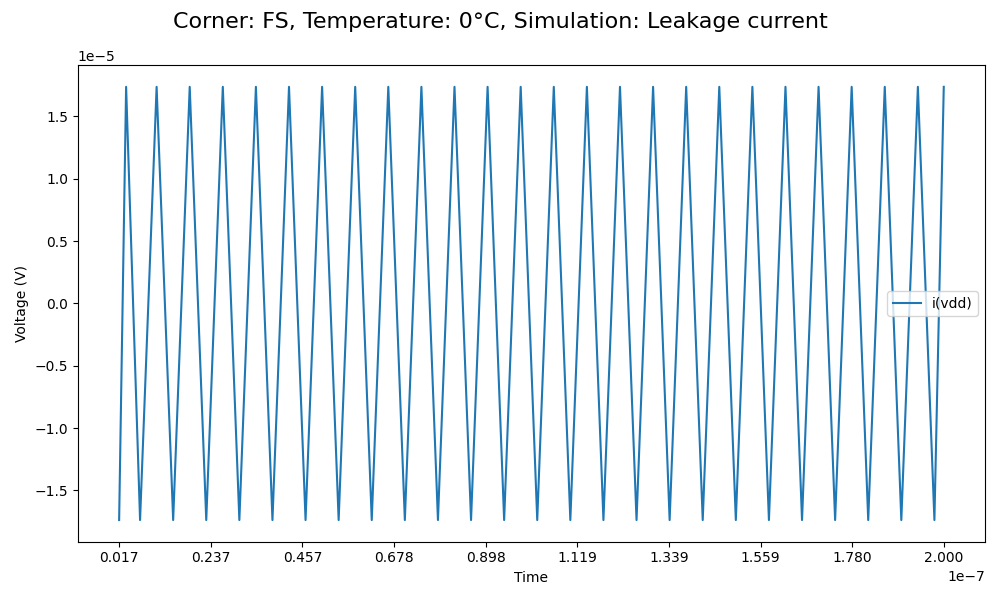
\includegraphics[height= 0.21\textheight]{figures/aimspice/FS/0/I.csv.png}
    \vspace{5pt}
    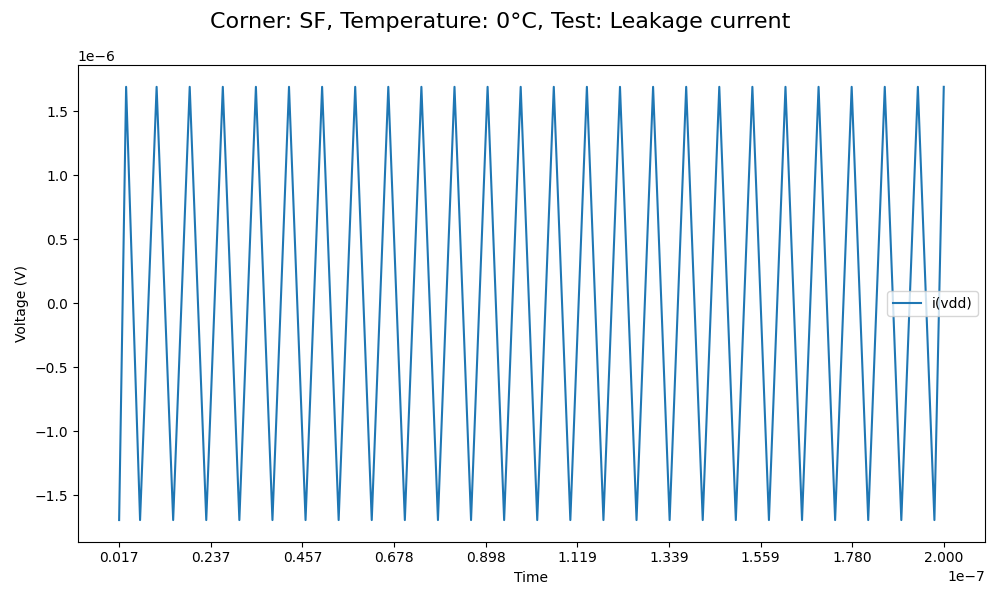
\includegraphics[height= 0.21\textheight]{figures/aimspice/SF/0/I.csv.png}
    \vspace{5pt}
    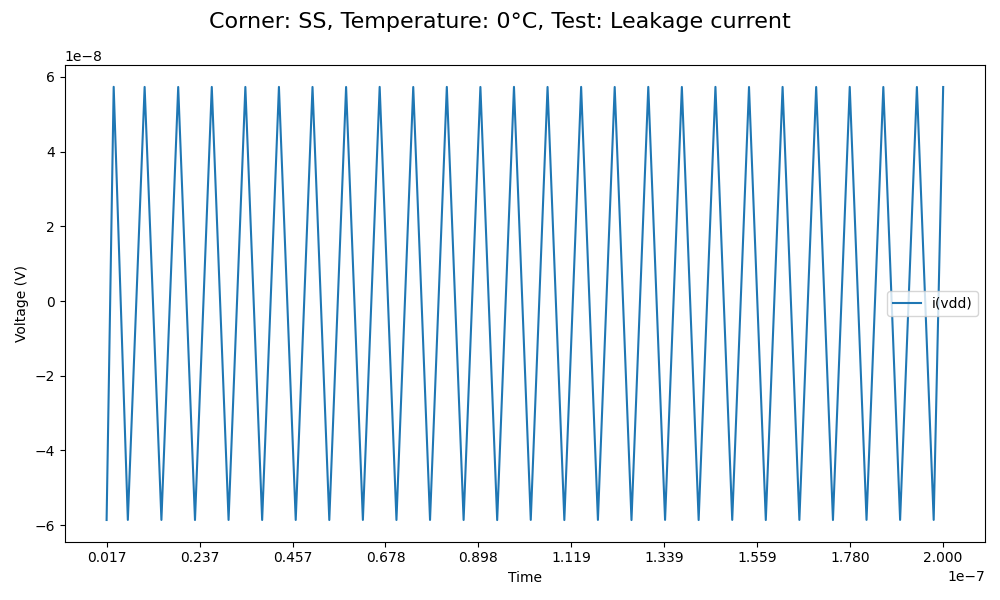
\includegraphics[height= 0.21\textheight]{figures/aimspice/SS/0/I.csv.png}
    \caption{Test of leakage current at 0 degrees celcius.}
    \label{fig:aimspice_I_0}
\end{figure}

\pagebreak

\begin{figure}[H]
    \centering
    \includegraphics[height= 0.21\textheight]{figures/aimspice/TT/27/I.csv.png}
    \vspace{5pt}
    \includegraphics[height= 0.21\textheight]{figures/aimspice/FF/27/I.csv.png}
    \vspace{5pt}
    \includegraphics[height= 0.21\textheight]{figures/aimspice/FS/27/I.csv.png}
    \vspace{5pt}
    \includegraphics[height= 0.21\textheight]{figures/aimspice/SF/27/I.csv.png}
    \vspace{5pt}
    \includegraphics[height= 0.21\textheight]{figures/aimspice/SS/27/I.csv.png}
    \caption{Test of leakage current at 27 degrees celcius.}
    \label{fig:aimspice_I_27}
\end{figure}

\pagebreak

\begin{figure}[H]
    \centering
    \includegraphics[height= 0.21\textheight]{figures/aimspice/TT/70/I.csv.png}
    \vspace{5pt}
    \includegraphics[height= 0.21\textheight]{figures/aimspice/FF/70/I.csv.png}
    \vspace{5pt}
    \includegraphics[height= 0.21\textheight]{figures/aimspice/FS/70/I.csv.png}
    \vspace{5pt}
    \includegraphics[height= 0.21\textheight]{figures/aimspice/SF/70/I.csv.png}
    \vspace{5pt}
    \includegraphics[height= 0.21\textheight]{figures/aimspice/SS/70/I.csv.png}
    \caption{Test of leakage current at 70 degrees celcius.}
    \label{fig:aimspice_I_70}
\end{figure}

